\documentclass[12pt]{article}

\usepackage{sbc-template}
\usepackage{graphicx,url}
\usepackage[utf8]{inputenc}
\usepackage[brazil]{babel}
\usepackage[latin1]{inputenc}  
\usepackage{booktabs}
\usepackage{amsmath}
\usepackage{float}
\usepackage{subcaption}
\usepackage{xcolor}

     
\sloppy

\title{Comparação de algoritmos de busca no jogo Othello: Minimax e Monte Carlo Tree Search}

\author{Jaime Antonio Daniel Filho\inst{1}, Diego Ribeiro Chaves\inst{1}}


\address{Curso de Ciência da Computação -- Universidade Federal de Santa Maria
  (UFSM)
  \email{jafilho@inf.ufsm.br, drchaves@inf.ufsm.br}
}

\begin{document} 

\maketitle

% ============================================================
\section{Introdução}
% ============================================================
 
Os jogos de tabuleiro de dois jogadores
%bipartidários 
têm servido como ambientes ideais para o
desenvolvimento e refinamento de algoritmos de decisão em inteligência artificial.
%desde os primórdios da computação.
A natureza determinística, de informação perfeita e adversarial
desses jogos oferece um domínio controlado onde é possível medir com precisão a qualidade das
decisões tomadas por diferentes agentes. O Othello, também conhecido como Reversi, é um exemplo
desse tipo de jogo, distinguindo-se de outros jogos de tabuleiro clássicos
por sua natureza dinâmica e pela dificuldade de estabelecer vantagem material cedo.
Diferentemente do xadrez, em que peças de diferentes valores podem ser trocadas, no Othello, todas
as peças são equivalentes e ganham ou perdem valor conforme sua posição no tabuleiro evolui.
Essa característica torna o jogo particularmente desafiador para algoritmos baseados em
heurísticas, pois o valor de uma posição não pode ser determinado exclusivamente pela contagem
de peças, mas depende de fatores posicionais complexos como controle de bordas, proximidade
dos cantos e mobilidade.

Neste trabalho, apresentar-se-a um estudo sistemático dos algoritmos de busca Minimax com poda alfa-beta e MCTS, com diferentes heurísticas e parâmetros de avaliação. Serão apresentados os resultados de extensivas simulações, contabilizando taxa de vitória, tempo médio por movimento, frequência de jogadas e capturas tanto na variante tradicional do jogo como na variante proposta.
 
% A escolha do Othello como domínio de estudo deve-se a propriedades que o tornam um intermediário
% ideal entre jogos simples e aqueles com espaços de estados astronomicamente grandes. O tabuleiro
% de $6\!\times\!6$ casas utilizado nesta investigação permite experimentos computacionalmente
% viáveis com múltiplos parâmetros, ao mesmo tempo em que preserva as complexidades estratégicas
% essenciais do jogo completo. A inclusão de uma variante circular (\emph{WrapAround}) adiciona
% uma camada adicional de interesse, modificando fundamentalmente as linhas de captura e
% eliminando as vantagens tradicionais associadas às posições de canto.
 
% ============================================================
% \section{Objetivos}
% % ============================================================
 
% Este trabalho tem como objetivo principal realizar uma comparação sistemática entre dois
% algoritmos para tomada de decisão em jogos de tabuleiro. O algoritmo Minimax com
% poda alfa-beta, representante clássico da busca determinística em árvores de jogo, e o MCTS,
% representante da busca probabilística baseada em simulações. A comparação busca identificar
% as condições em que cada abordagem oferece vantagens perceptíveis, em termos de taxa de vitória
% e de eficiência computacional.
 
% Além disso, visa-se examinar como diferentes funções de avaliação afetam o
% desempenho do Minimax, desde avaliadores simples baseados em contagem de material até
% avaliadores sofisticados que combinam múltiplos fatores posicionais e são ajustados por
% aprendizado de máquina. A investigação também busca compreender como a profundidade de busca
% no Minimax e o número de iterações no MCTS influenciam a qualidade das decisões e o custo
% computacional. Além disso, implementou-se uma variante do jogo, com capturas circulares nas casas do canto do tabuleiro, o que trouxe um novo paradigma de estratégias e jogadas ideais.
% nas estratégias ótimas, verificando se avaliadores treinados no jogo clássico se transferem para a nova variante.
 
% ============================================================
\section{O jogo Othello}
% ============================================================
 
O Othello é jogado em um tabuleiro quadrado dividido em casas iguais. Neste estudo, utilizar-se-a
a variante com tabuleiro de $6\!\times\!6$ casas, diferentemente do Othello padrão que emprega
tabuleiros de $8\!\times\!8$. A configuração inicial do jogo clássico apresenta quatro peças
posicionadas no centro do tabuleiro, formando um quadrado com duas peças de cada cor dispostas
em diagonal. O mecanismo central de captura baseia-se no princípio do flanqueamento. Uma peça
é capturada quando fica completamente envolvida por peças do oponente em uma linha reta, seja
horizontal, vertical ou diagonal. Para que uma jogada seja legal, ela deve resultar em pelo menos
uma captura em qualquer das oito direções possíveis.
 
Uma regra fundamental determina que, se um jogador não possui nenhum movimento legal disponível,
ele passa a vez para o oponente. A partida termina quando nenhum dos dois jogadores consegue
realizar um movimento legal, e o vencedor é determinado pela contagem final de peças. A
Figura~\ref{fig:classical_board} ilustra o estado inicial do jogo clássico na interface
implementada neste trabalho.
 
\begin{figure}[H]
  \centering
  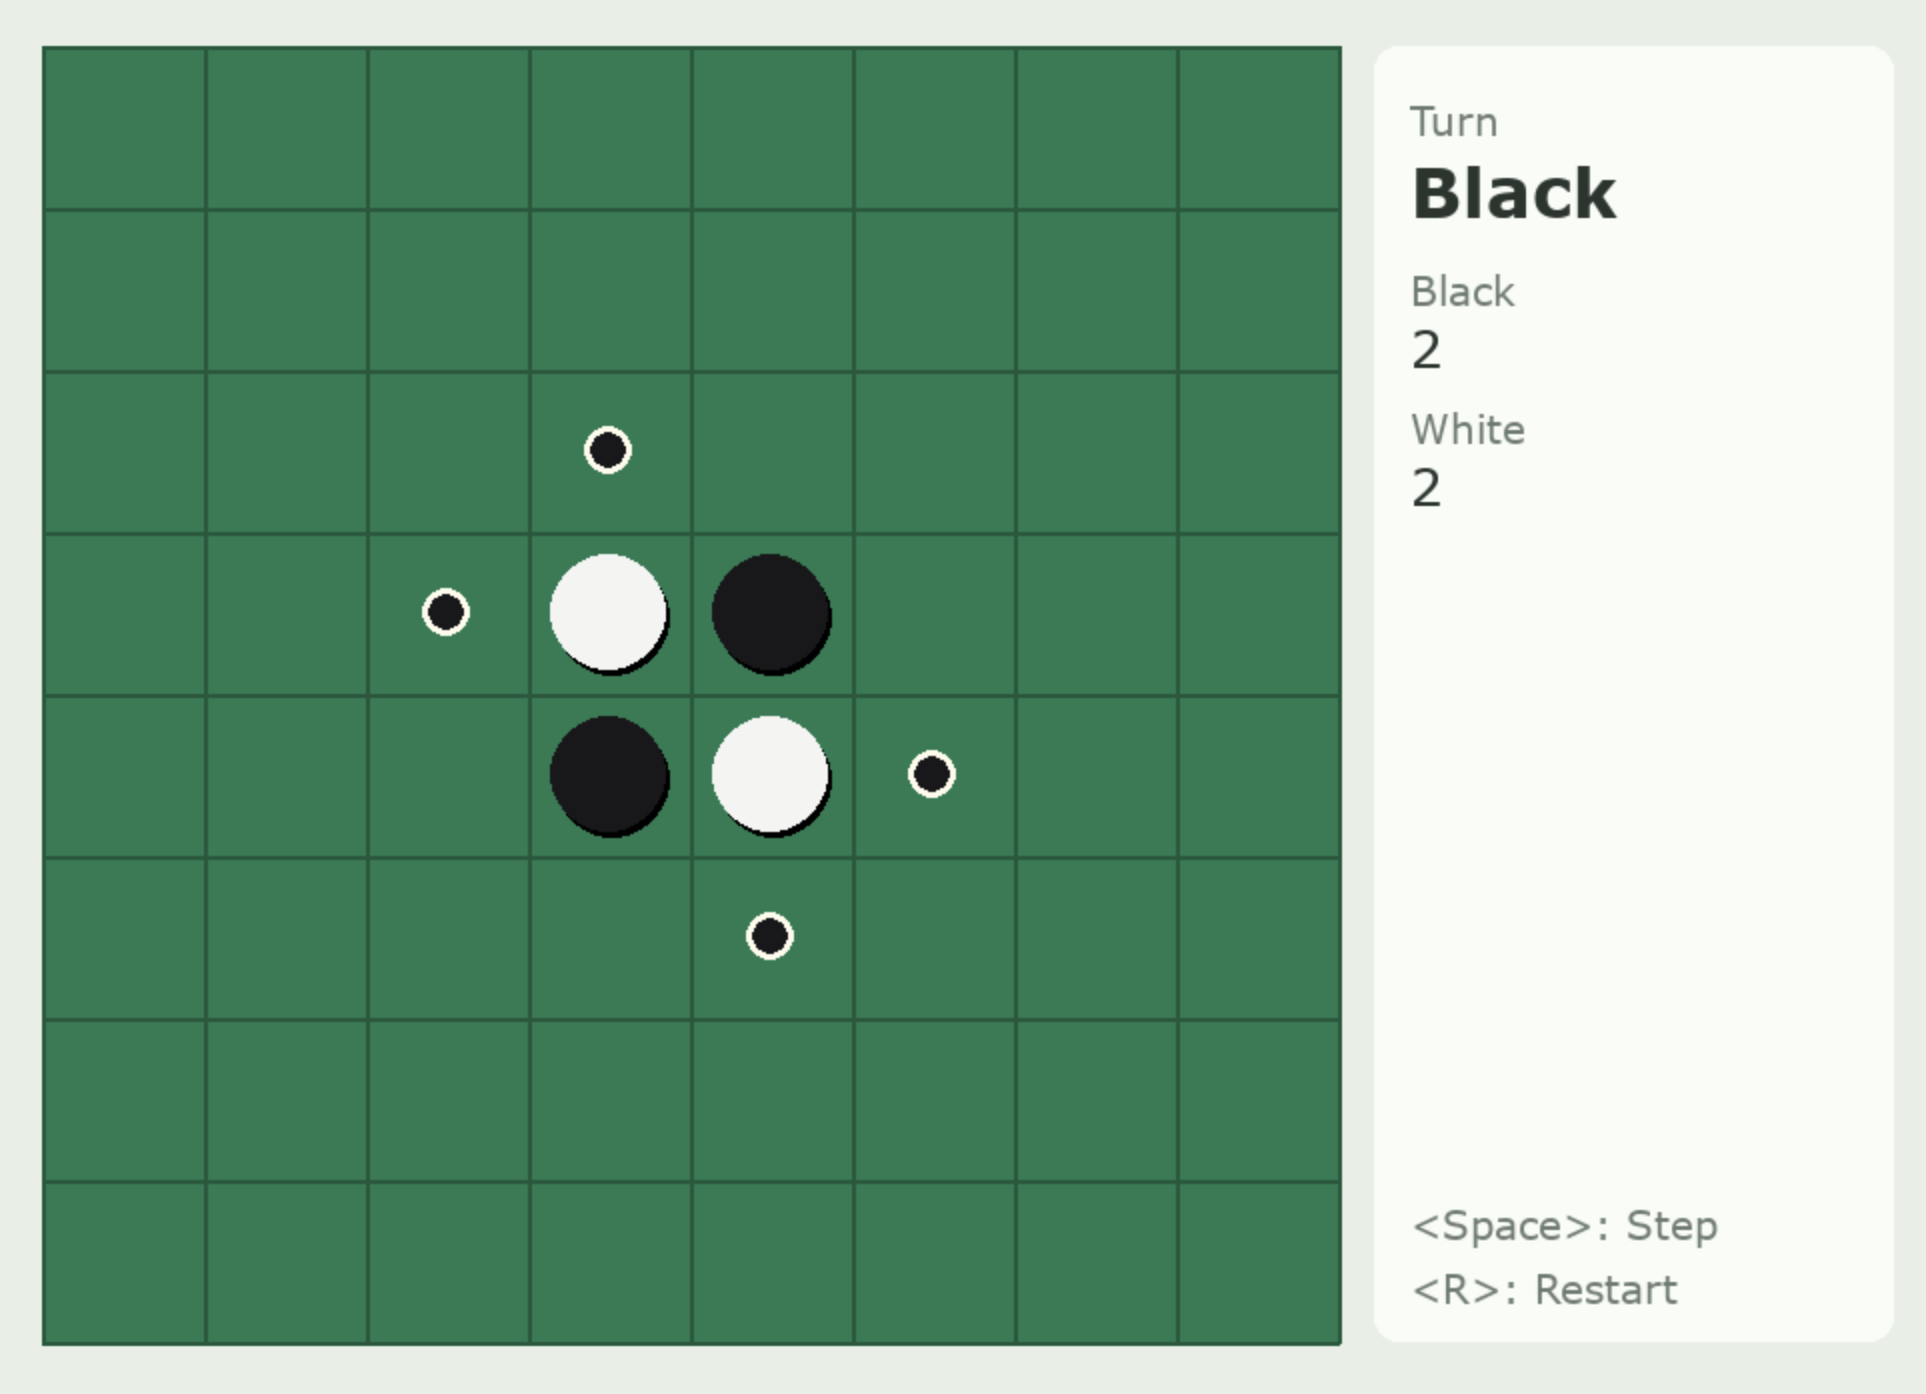
\includegraphics[width=0.55\textwidth]{classical_board.png}
  \caption{Posição inicial do jogo clássico na interface da implementação. %As quatro peças
    %centrais formam o padrão tradicional de abertura, com pretas iniciando a partida.
    }
  \label{fig:classical_board}
\end{figure}
 
A hierarquia posicional no Othello clássico é bem estabelecida. Os cantos do tabuleiro
representam as posições de maior valor estratégico, pois uma vez ocupados permanecem
permanentemente sob controle do jogador que os conquistou, já que não é possível flanquear
uma peça a partir do canto em múltiplas direções. As casas adjacentes aos cantos, posições
C e X, representam o oposto, isto é, ocupá-las cria oportunidades para o oponente capturar
os cantos adjacentes, sendo portanto posições de risco. As bordas do tabuleiro,
excluindo cantos e adjacências, oferecem vantagens moderadas, conferindo controle parcial
sobre linhas de captura.

A Figura~\ref{fig:board_value} apresenta o rótulo das casas inicialmente definidos com base no livro A Minute to Learn... A Lifetime to Master - Brian Rose.

\begin{figure}[H]
  \centering
  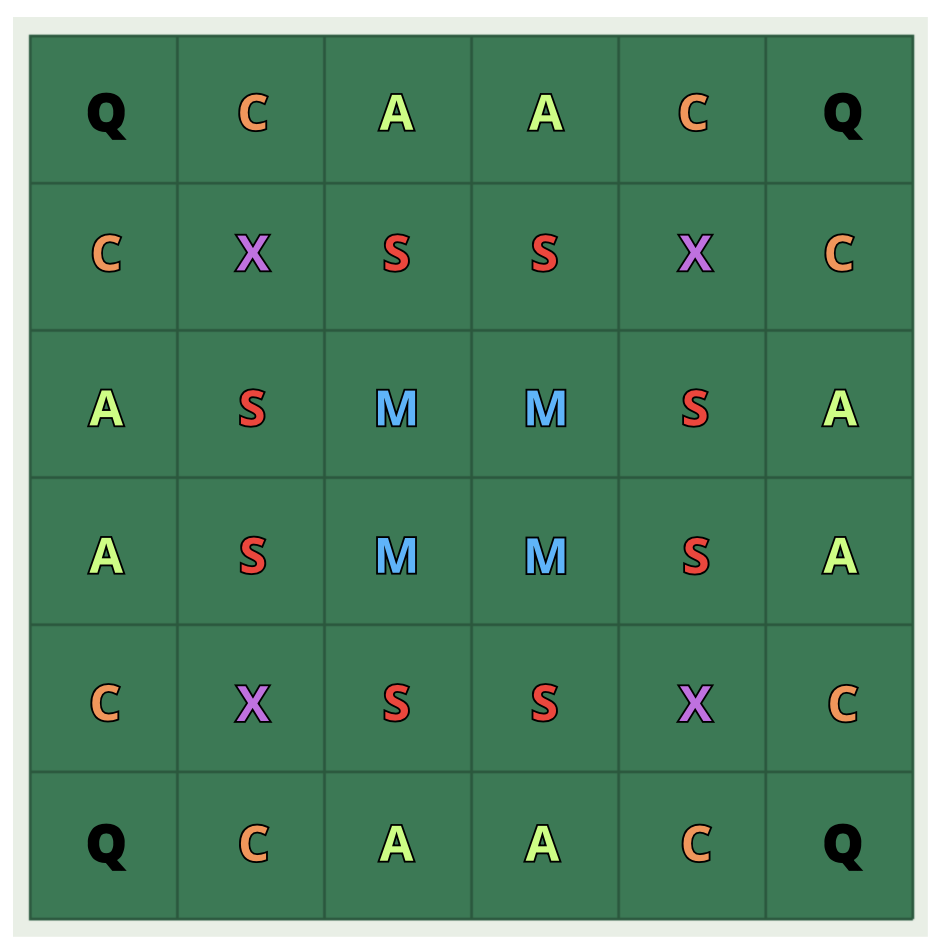
\includegraphics[width=0.45\textwidth]{board_value.png}
  \caption{Rótulo das casas no tabuleiro do jogo.
    }
  \label{fig:board_value}
\end{figure}

 
\subsection{Variante Circular}



Na variante circular, proposta para este trabalho, as quatro peças
iniciais são posicionadas nos cantos do tabuleiro, com duas brancas nos cantos superiores e
duas pretas nos cantos inferiores.
Além disso, as duas diagonais principais funcionam como portais
para acessar o lado oposto do tabuleiro. Isso significa que, se uma
peça está posicionada exatamente sobre uma das diagonais, a diagonal principal, canto
superior esquerdo ao canto inferior direito, ou a diagonal secundária, canto superior
direito ao canto inferior esquerdo, qualquer movimento a partir dela age como se as
bordas opostas estivessem conectadas, isto é, ao sair por uma borda, a linha de visão
reaparece na borda oposta, na mesma linha ou coluna. Para todas as outras casas, fora
dessas diagonais, o comportamento é o tradicional do Othello.
 
A Figura~\ref{fig:warp_board} apresenta a posição inicial da variante circular, evidenciando
a disposição diferenciada das peças nos cantos.
 
\begin{figure}[H]
  \centering
  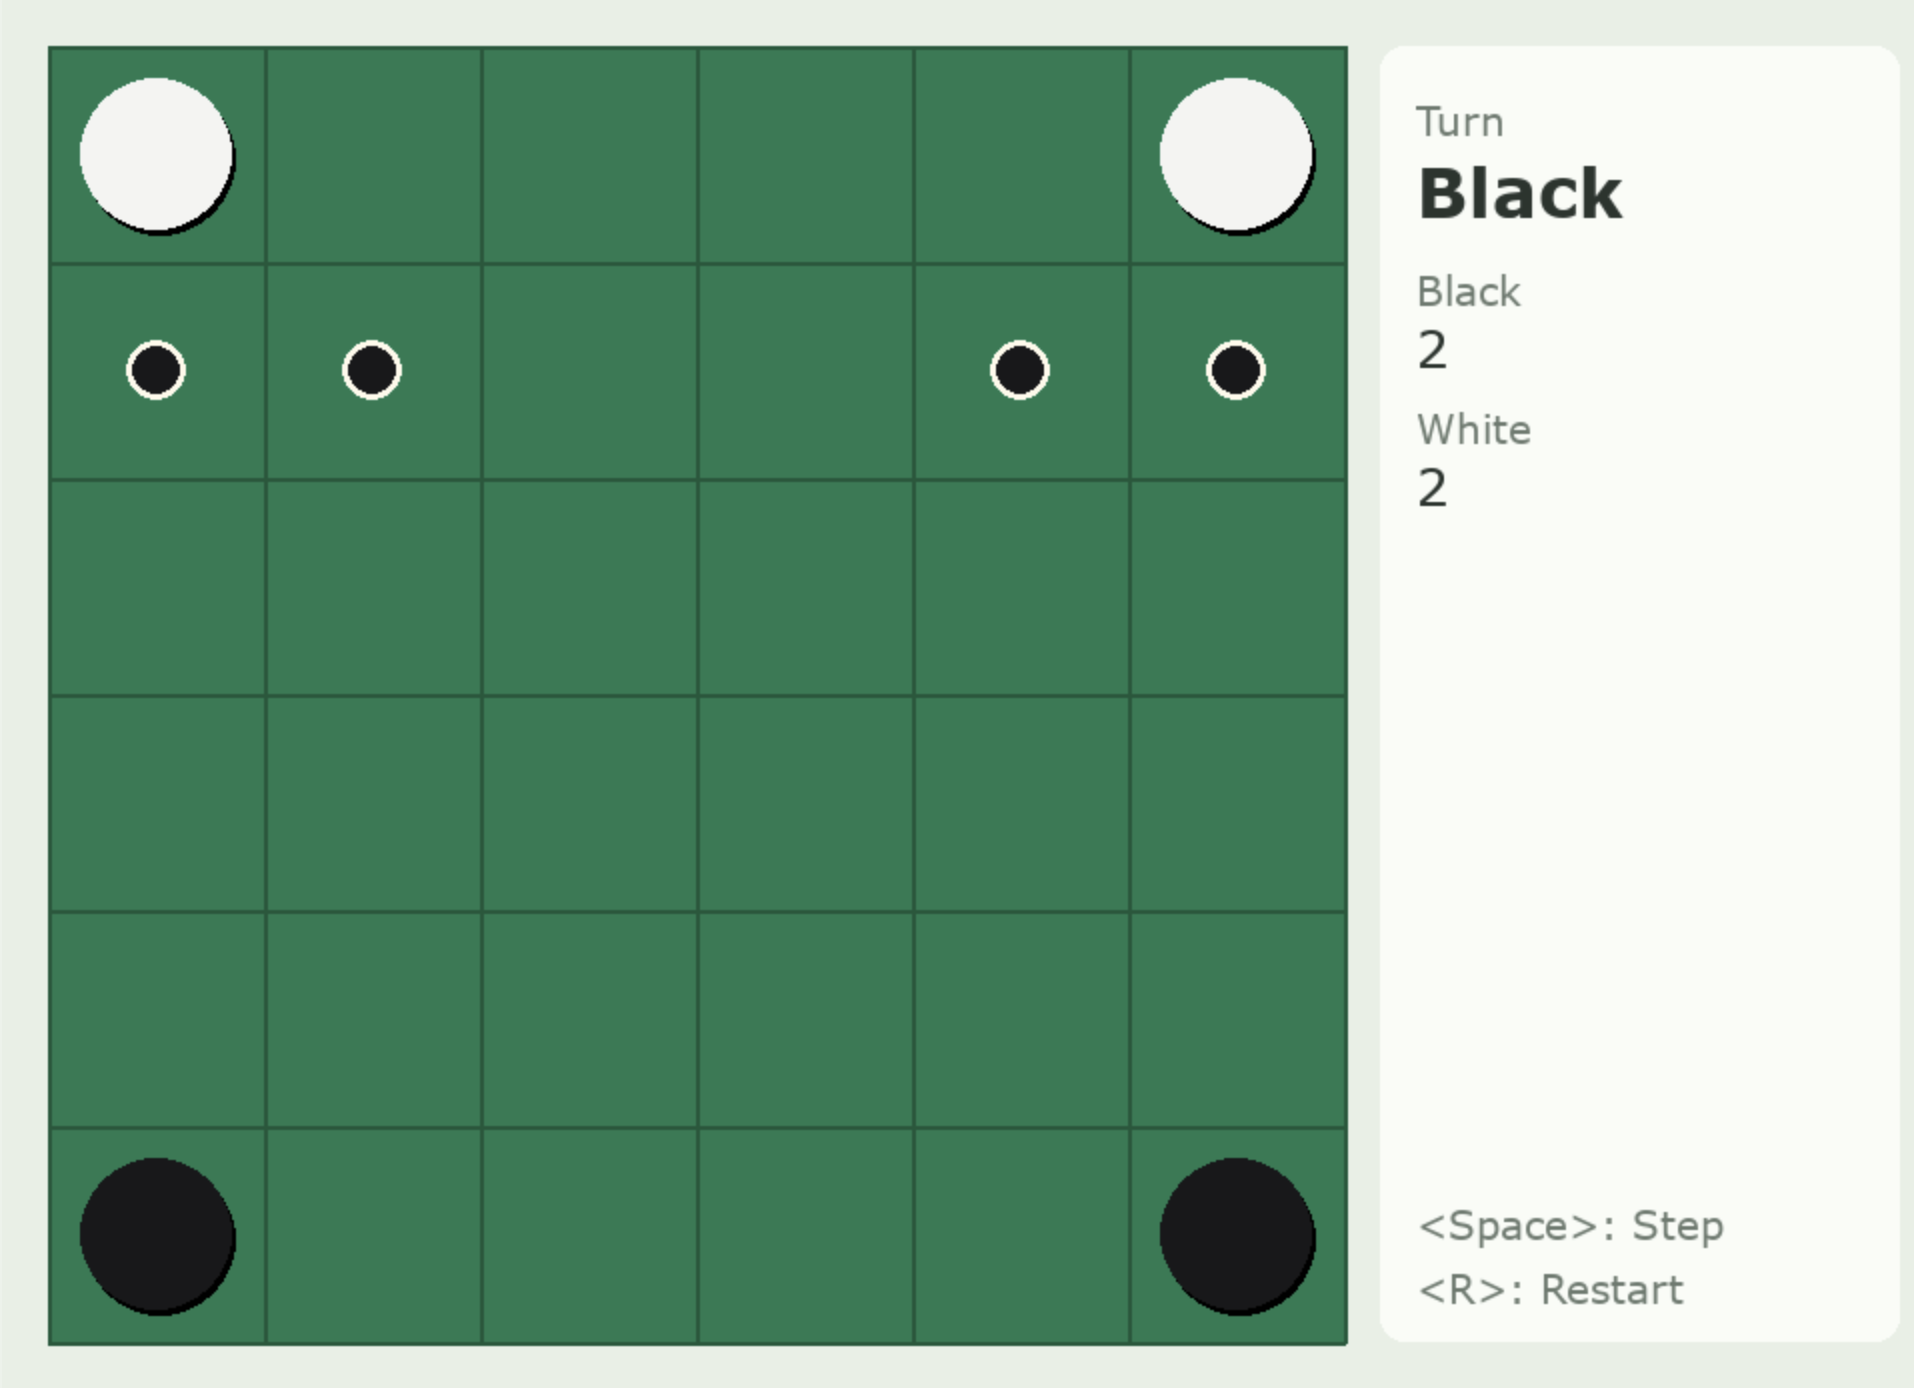
\includegraphics[width=0.55\textwidth]{warp_around_board.png}
  \caption{Posição inicial da variante circular na interface da implementação. 
  %As peças brancas
    %ocupam os cantos superiores e as pretas os cantos inferiores, criando uma abertura
    %radicalmente distinta da variante clássica.
    }
  \label{fig:warp_board}
\end{figure}
 
A Figura~\ref{fig:warp_captures} detalha os três tipos de capturas circulares que ocorrem nessa
variante. As flechas partem sempre dos cantos, que é o único lugar onde a circularidade pode se
manifestar. A imagem da esquerda mostra capturas nas diagonais, a do centro nas linhas dos cantos
e a da direita nas colunas dos cantos.
 
\begin{figure}[H]
  \centering
  \begin{subfigure}[b]{0.31\textwidth}
    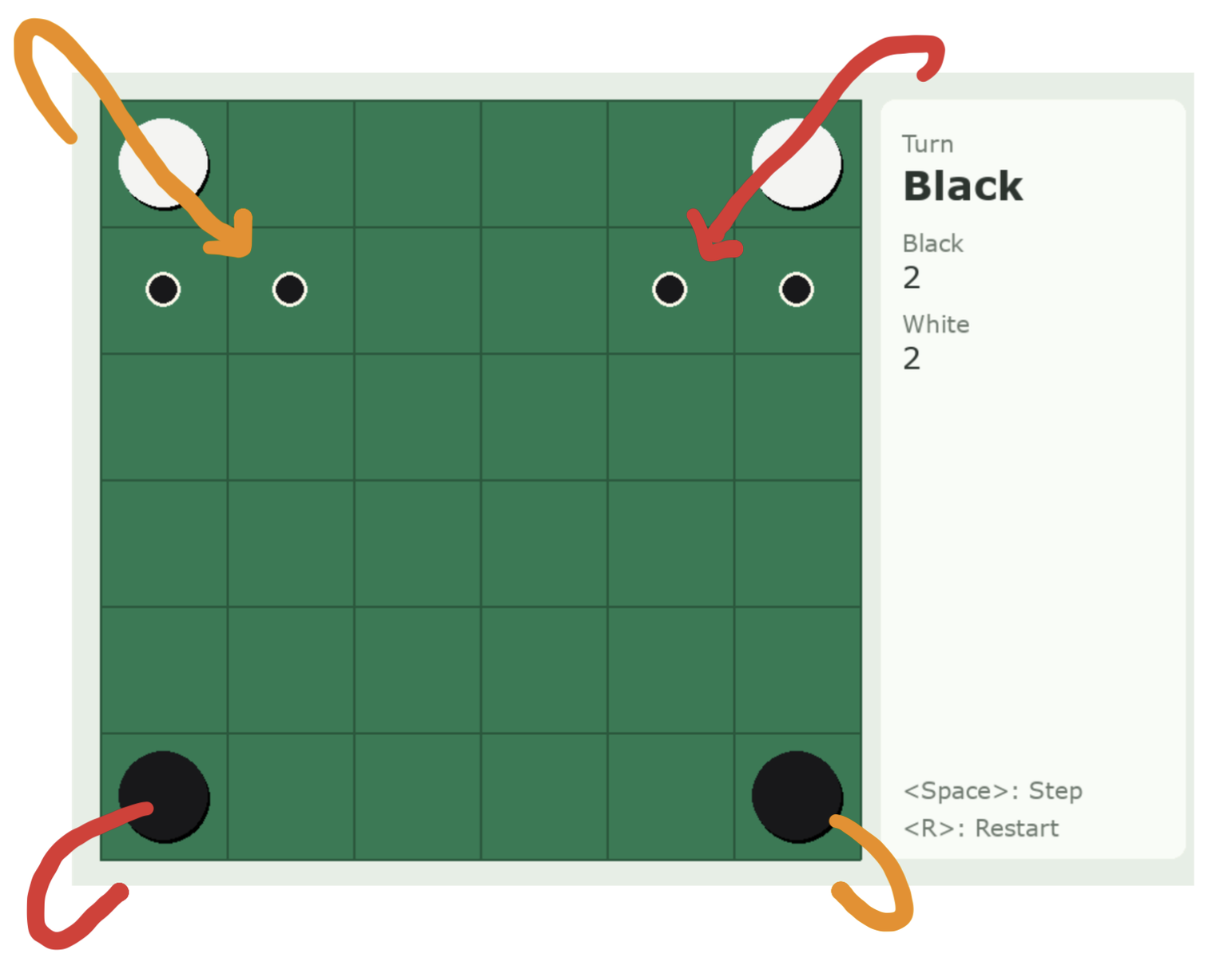
\includegraphics[width=\textwidth]{warp_around_board_1.png}
    \caption{Capturas diagonais.}
  \end{subfigure}
  \hfill
  \begin{subfigure}[b]{0.31\textwidth}
    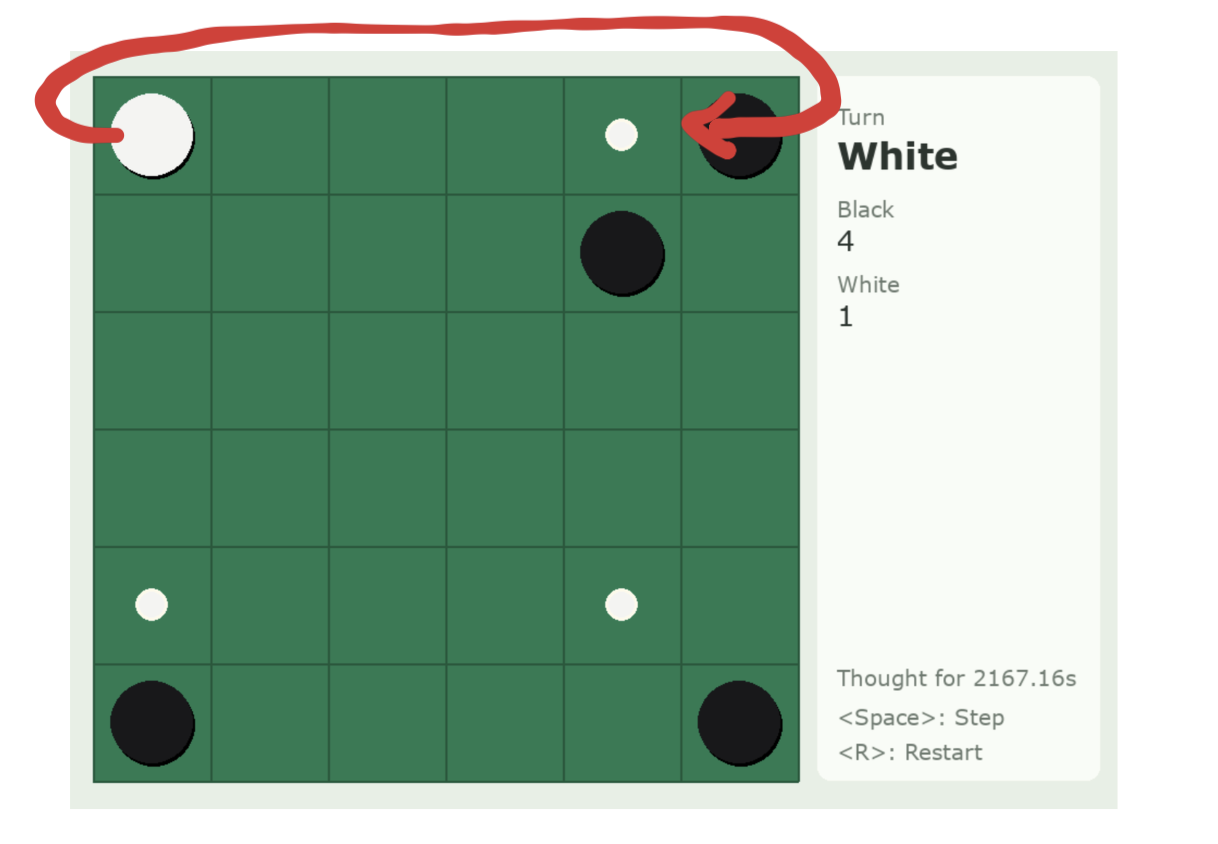
\includegraphics[width=\textwidth]{warp_around_board_2.png}
    \caption{Capturas nas linhas dos cantos.}
  \end{subfigure}
  \hfill
  \begin{subfigure}[b]{0.31\textwidth}
    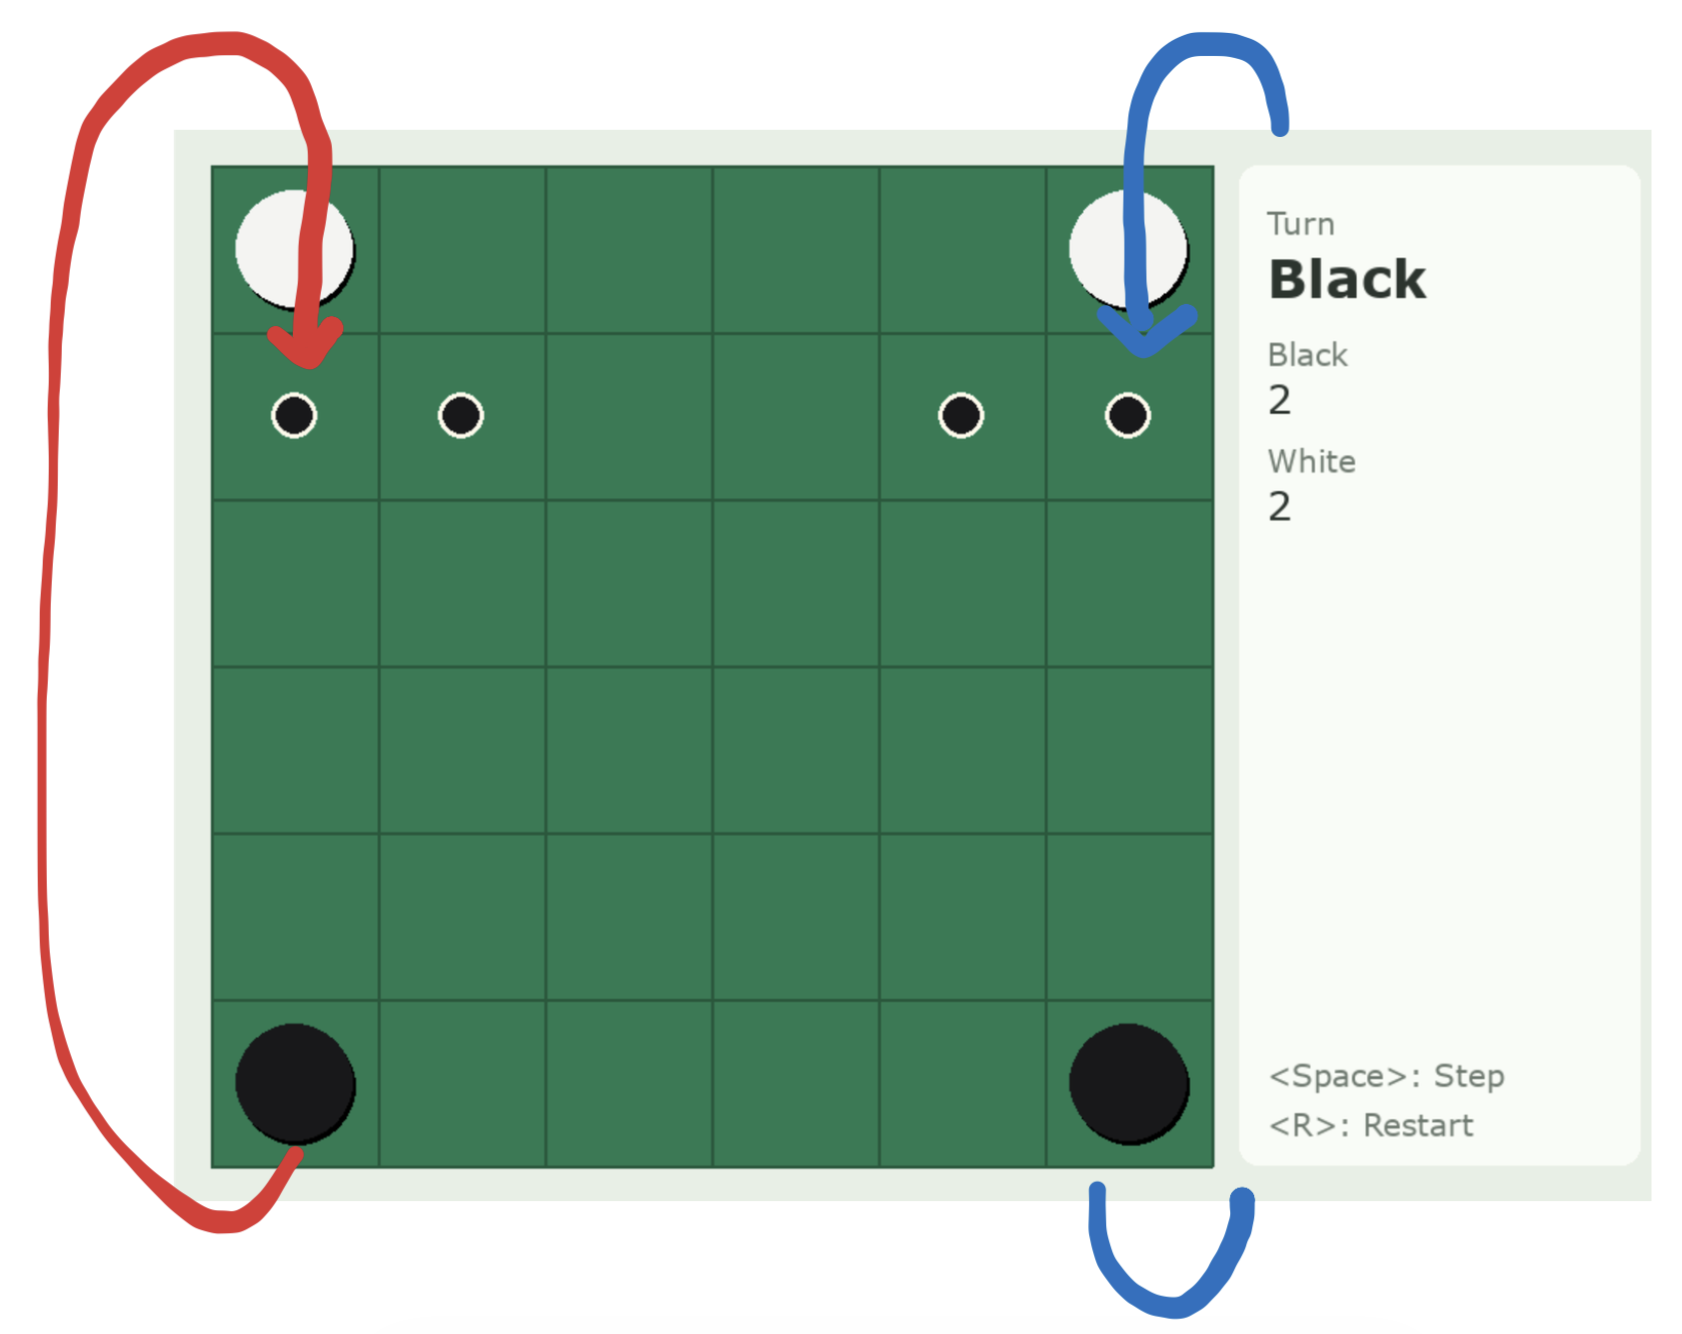
\includegraphics[width=\textwidth]{warp_around_board_3.png}
    \caption{Capturas nas colunas dos cantos.}
  \end{subfigure}
  \caption{Ilustração das capturas circulares na variante circular. As flechas partem
    dos cantos, o único lugar em que a circularidade pode ocorrer, e indicam as direções de
    visão que atravessam a borda do tabuleiro.}
  \label{fig:warp_captures}
\end{figure}
 
Isso implica que
peças sobre as diagonais principais ganham linhas de captura que podem atravessar
o tabuleiro de forma circular. Uma peça num canto, por exemplo, deixa de ter apenas
três direções limitadas e passa a enxergar o lado oposto inteiro.
Com isso, estratégias de canto e de borda mudam radicalmente, pois um canto está sempre sobre
pelo menos uma diagonal. Isso torna os cantos portas de entrada para ataques que atravessam o centro do tabuleiro. Ainda, a propagação de viradas de peças pode formar laços inesperados. Por exemplo,
uma fileira de peças do adversário pode ser flanqueada por uma peça sua que está do outro lado do tabuleiro,  desde que a casa de partida esteja sobre uma diagonal.
 
% ============================================================
\section{Agentes}
% ============================================================
 
\subsection{Monte Carlo Tree Search (MCTS)}
 
O algoritmo MCTS representa uma abordagem fundamentalmente diferente para tomada de decisão
em jogos, abandonando a avaliação explícita de posições em favor de amostragem estatística
através de simulações aleatórias. Desde sua introdução e seu subsequente sucesso no jogo de
Go, o MCTS tornou-se uma técnica amplamente utilizada.
 
O algoritmo opera através de quatro fases que se repetem iterativamente até que o critério de
parada seja satisfeito. Neste trabalho, um número fixo de iterações. A seleção percorre a árvore a partir
da raiz utilizando a fórmula UCT (\textit{Upper Confidence Bound for Trees}), que balanceia
exploração e explotação. Os nós menos visitados recebem um bônus de exploração que aumenta com visitas adicionais ao nó pai e diminui conforme o próprio nó filho recebe mais visitas. A expansão ocorre
quando um nó ainda não foi completamente desenvolvido, sendo um dos movimentos não explorados
selecionado aleatoriamente e um novo nó filho é criado. A simulação
prossegue jogando aleatoriamente a partir do novo nó até atingir um estado terminal. A
retropropagação percorre o caminho inverso até a raiz, atualizando as estatísticas, como número de visitas e soma de vitórias e derrotas, de cada nó visitado.
 
Uma característica distintiva do MCTS é que ele não requer função de avaliação heurística
explícita, uma vez que a avaliação emerge das estatísticas acumuladas. Isso o torna adequado para domínios
onde heurísticas precisas são difíceis de formular, mas também significa que pode requerer
muitas iterações para atingir desempenho comparável ao Minimax configurado com boas
heurísticas.
 
\subsection{Minimax com Poda Alfa-Beta}
 
O algoritmo Minimax representa uma das abordagens clássicas para tomada de decisão em
jogos de soma zero. A estratégia assume que cada jogador busca maximizar sua própria vantagem
enquanto minimiza a do oponente. A implementação funciona explorando recursivamente a árvore de
jogo a partir do estado atual, alternando entre nós de maximização e minimização. Na profundidade
máxima, isto é, nos nós folha, uma função de avaliação heurística estima a qualidade da posição. Esse
valor é então propagado de volta. Em nós de maximização, o maior valor entre os filhos é
selecionado, ao passo que em nós de minimização, o menor. Dessa forma, o algoritmo assume que ambos os
jogadores jogam otimamente.
 
A poda alfa-beta constitui a principal otimização, permitindo eliminar subárvores que não podem
influenciar a decisão final. O mecanismo mantém dois valores, $\alpha$ (melhor garantido para
o maximizador) e $\beta$ (melhor garantido para o minimizador), e descarta nós sempre que
$\alpha \geq \beta$. A eficácia da poda depende da ordem em que os movimentos são
explorados. A Figura~\ref{fig:minimax_tree} ilustra uma execução do algoritmo Minimax com
indicação das podas realizadas.
 
\begin{figure}[H]
  \centering
  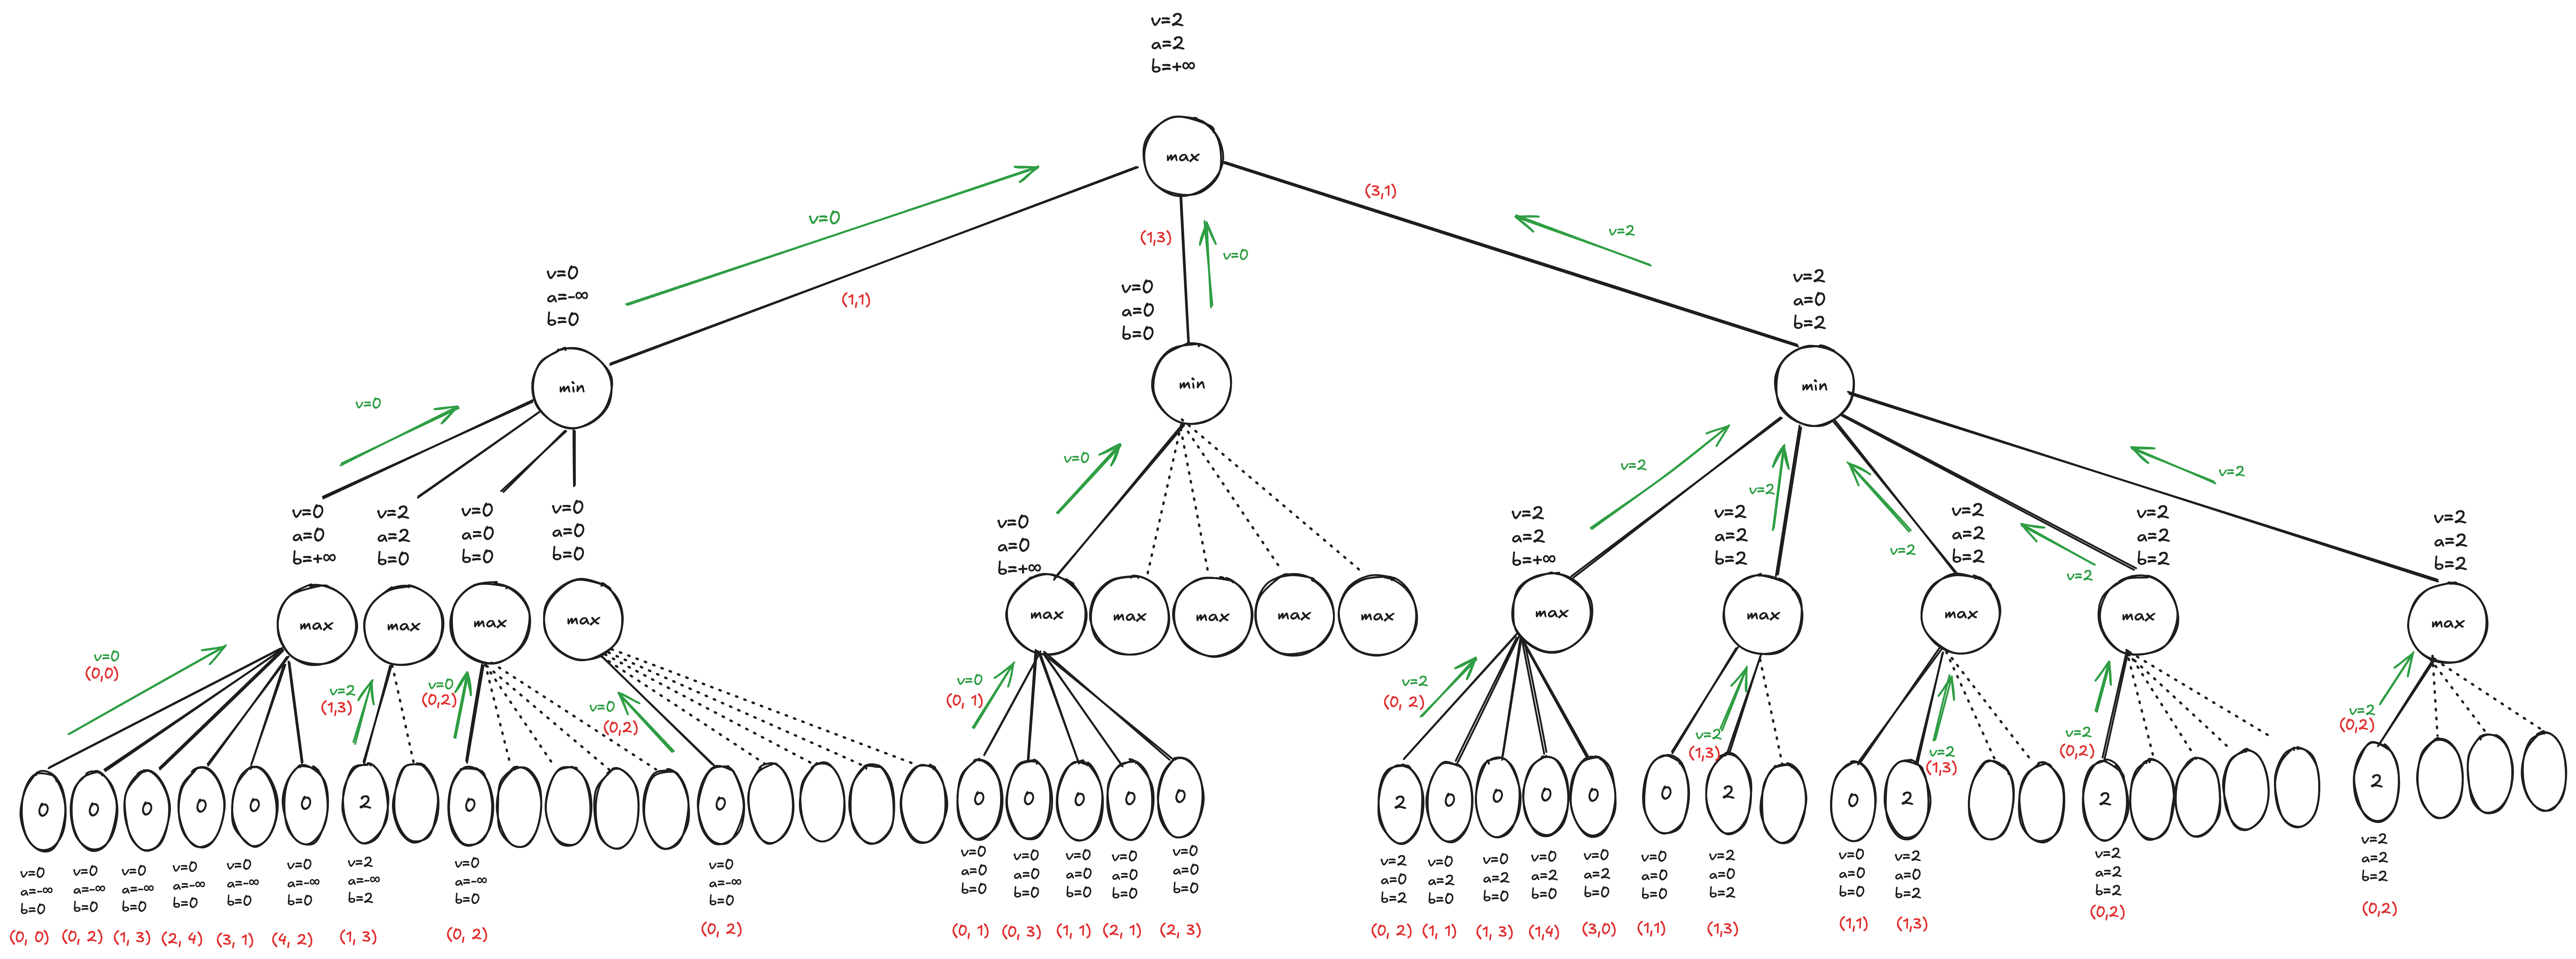
\includegraphics[width=0.72\textwidth]{minimax_manual.png}
  \caption{Árvore do Minimax com indicação dos nós podados. O valor do
    último nó corresponde ao resultado da função de avaliação de diferença de peças
    (brancas menos pretas). Em vermelho estão os movimentos na forma (linha, coluna).}
  \label{fig:minimax_tree}
\end{figure}
 
Neste trabalho, o Minimax foi avaliado com profundidades de 1 a 6. As métricas coletadas
incluem contadores de nós explorados e nós podados, permitindo analisar a eficácia da poda em
diferentes contextos.
 
% ============================================================
\section{Funções de Avaliação (Heurísticas)}
% ============================================================
 
A qualidade das decisões tomadas pelo Minimax depende criticamente da função de avaliação
empregada. O sistema de pesos adotado segue uma arquitetura unificada onde cada avaliador mantém
um vetor de pesos que indica a importância relativa de diferentes parâmetros extraídos do estado.
A pontuação final é o produto interno entre o vetor de pesos e o vetor de parâmetros:
\begin{equation}
  v(s) = \mathbf{w}^\top \boldsymbol{\phi}(s),
  \label{eq:eval}
\end{equation}
onde $\mathbf{w}$ é o vetor de pesos e $\boldsymbol{\phi}(s)$ é o vetor de características do
estado $s$. Todas as avaliações são feitas do ponto de vista das peças brancas, ou seja, valores positivos
indicam vantagem para as brancas e negativos, para as pretas.
 
\subsection{Heurística de Material}
 
O avaliador de contagem de peças representa a heurística mais elementar,
quantificando a vantagem material direta. Dois parâmetros são calculados, normalizados pelo
total de casas:
\begin{equation}
  \phi_{\text{mat}} = \left(\frac{N_W}{36},\; \frac{N_B}{36}\right),
\end{equation}
onde $N_W$ e $N_B$ são os totais de peças brancas e pretas, respectivamente. Com os pesos
padrão $\mathbf{w} = [1{,}0,\; {-}1{,}0]$, a avaliação retorna simplesmente a diferença
normalizada entre peças brancas e pretas. Embora simples, este avaliador não considera a qualidade posicional das peças nem fatores dinâmicos como
mobilidade e controle de espaço, sendo especialmente fraco nas fases iniciais do jogo.
 
\subsection{Heurística de Posição}
 
O avaliador posicional divide o tabuleiro $6\!\times\!6$ em seis
regiões com propriedades estratégicas distintas:
 
\begin{table}[H]
  \centering
  \caption{Regiões do tabuleiro e respectivos pesos padrão para o avaliador posicional.}
  \label{tab:regions}
  \begin{tabular}{clcc}
    \toprule
    Região & Casas & Peso (brancas) & Peso (pretas) \\
    \midrule
    Q (cantos) & $(0,0),(0,5),(5,0),(5,5)$ & $+1{,}00$ & $-1{,}00$ \\
    C (adj.\ cantos) & bordas adjacentes aos cantos & $-0{,}25$ & $+0{,}25$ \\
    X (diag.\ cantos) & $(1,1),(1,4),(4,1),(4,4)$ & $-0{,}50$ & $+0{,}50$ \\
    A (bordas centrais) & bordas exceto cantos e adj. & $+0{,}10$ & $-0{,}10$ \\
    S (anel interno) & anel interno próximo ao centro & $+0{,}05$ & $-0{,}05$ \\
    M (centro) & casas centrais & $+0{,}01$ & $-0{,}01$ \\
    \bottomrule
  \end{tabular}
\end{table}
 
Para cada região $i$, calculam-se as frações de peças brancas e pretas presentes, gerando
um vetor de $12$ parâmetros. Os pesos padrões refletem a estratégica clássica, em que cantos são
estáveis e portanto muito valiosos, as casas C e X são perigosas, pois facilitam ao oponente
capturar os cantos adjacentes.
 
\subsection{Heurística de Mobilidade Potencial}
 
O avaliador de mobilidade potencial captura o conceito
de peças fronteiriças. Uma peça é considerada fronteiriça se está adjacente a pelo menos
uma casa vazia. 
%O princípio subjacente é que peças no interior, sem contato com casas vazias, oferecem mais mobilidade ao oponente.
São calculados dois parâmetros normalizados:
\begin{equation}
  \phi_{\text{mob}} = \left(\frac{F_W}{36},\; \frac{F_B}{36}\right),
\end{equation}
onde $F_W$ e $F_B$ são o número de peças fronteiriças de cada cor. Com pesos padrão
$[-1{,}0,\; +1{,}0]$, o avaliador penaliza ter muitas peças brancas na fronteira e premia
ter muitas pretas na fronteira, capturando o objetivo de maximizar a mobilidade adversária e reduzir a própria.
 
\subsection{Heurística de Paridade}
 
O avaliador de paridade captura a vantagem do último movimento.
O jogador que realiza a última jogada tem vantagem decisiva, podendo converter peças
remanescentes do oponente. O avaliador retorna $1{,}0$ se a paridade atual desfavorece as
brancas, ou seja, o número de casas vazias é par e é vez das brancas, ou ímpar e é vez das
pretas, e $0{,}0$ caso contrário. Um único peso de $-1{,}0$ escalona essa contribuição.
 
\subsection{Composição de Heurísticas}
 
Dois mecanismos de composição são utilizados. O avaliador composto simplesmente
concatena os parâmetros e pesos de múltiplos avaliadores independentes, permitindo criar
avaliações complexas a partir de componentes simples. A avaliação composta é a soma das
avaliações individuais. O avaliador baseado em fases divide a partida em três fases
baseadas no número de casas vazias:
 
\begin{itemize}
  \item \textbf{Abertura}: mais de 22 casas vazias.
  \item \textbf{Meio-jogo}: entre 11 e 22 casas vazias.
  \item \textbf{Fim de jogo}: até 10 casas vazias.
\end{itemize}
 
Cada fase possui um avaliador composto independente com seus próprios pesos. Apenas o avaliador
da fase ativa contribui para a pontuação, enquanto os demais têm parâmetros zerados, permitindo que
diferentes fatores sejam priorizados ao longo da partida.
 
\subsection{Definição dos Avaliadores}
 
Seis avaliadores foram definidos e avaliados neste estudo, organizados em dois grupos: os
avaliadores para a variante clássica e os avaliadores para a variante circular.
 
\paragraph{SCE1 - Simple Count Evaluator 1.}
O avaliador mais simples, constituído exclusivamente de um %\texttt{CountEvaluator} com pesos
avaliador de contagem de peças padrão com pesos $[1{,}0,\; {-}1{,}0]$. Não possui sensibilidade à fase do jogo e ignora qualquer
fator posicional ou de mobilidade. Serve como linha de base para comparação com os demais.
 
\paragraph{CEE1 - Classical Empiric Evaluator 1.}
Avaliador sensível à fase do jogo com pesos escolhidos empiricamente. Cada fase combina
%\texttt{PositionalEvaluator}, \texttt{CountEvaluator} e \texttt{PotentialMobilityEvaluator}
a avaliação posicional, de contagem e de mobilidade potencial
com os seguintes pesos de escala:
\begin{itemize}
  \item \textbf{Abertura}: Posição $\times 0{,}4$ + Material $\times 0{,}2$ +
    Mobilidade $\times 0{,}2$.
  \item \textbf{Meio-jogo}: Posição $\times 0{,}3$ + Material $\times 0{,}4$ +
    Mobilidade $\times 0{,}2$.
  \item \textbf{Fim de jogo}: Material $\times 0{,}7$ + Posição $\times 0{,}2$ +
    Mobilidade $\times 0{,}1$.
\end{itemize}
Notavelmente, o CEE1 não inclui o 
%\texttt{ParityEvaluator},
avaliador de paridade, uma omissão que pode limitar
seu desempenho no fim de jogo. Os pesos foram definidos intuitivamente, sem otimização
baseada em dados.
 
\paragraph{CSTE1 - Classical Score-Tuned Evaluator 1.}
Avaliador sensível à fase treinado por regressão linear para prever a pontuação
final da partida, isto é, a diferença de peças. Cada fase combina %\texttt{CountEvaluator},
%\texttt{PositionalEvaluator}, \texttt{PotentialMobilityEvaluator} e \texttt{ParityEvaluator}.
avaliador de contagem, posicional, de mobilidade e de paridade.
O dataset de treinamento foi construído com partidas MCTS(10\,000) vs.\ MCTS(10\,000),
incluindo 0 a 7 movimentos aleatórios iniciais, totalizando 700 partidas, 20\,065
movimentos e ${\approx}57$ horas de simulação. Os pesos aprendidos diferem
substancialmente dos valores intuitivos do CEE1, especialmente para o 
%\texttt{PositionalEvaluator},
avaliador posicional
onde algumas regiões recebem pesos inesperadamente grandes, como $65{,}6$ para cantos das
brancas na abertura.
 
\paragraph{CWTE1 - Classical Win-Tuned Evaluator 1.}
Avaliador sensível à fase treinado por regressão logística para prever vitória ou
derrota. Mesma estrutura de componentes que o CSTE1, mas com pesos otimizados para maximizar a probabilidade de vitória. Utiliza o mesmo
dataset também. No meio-jogo, o
%\texttt{PotentialMobilityEvaluator}
avaliador de mobilidade potencial recebe pesos de
($[-5{,}14,\; 5{,}78]$), indicando que ter muitas peças brancas na fronteira é prejudicial,
o que está alinhado com a estratégia de minimizar a exposição.
 

 
\paragraph{WSTE1 - Wrap Around Score-Tuned Evaluator 1.}
Análogo ao CSTE1, mas treinado por regressão linear na variante circular. O dataset foi construído com partidas MCTS(5\,000) vs.\ MCTS(5\,000), totalizando
$2\,700$ partidas, 76\,975 movimentos e ${\approx}104$ horas de simulação. Apresenta pesos de maior magnitude, especialmente para o 
%\texttt{PositionalEvaluator}
avaliador posicional
no meio-jogo, com valores como $+24{,}2$ para regiões C das brancas, confirmando a
redistribuição de importância posicional nessa variante.

\paragraph{WWTE1 - Wrap Around Win-Tuned Evaluator 1.}
Análogo ao CWTE1, mas treinado com regressão logística especificamente na variante
circular com o mesmo dataset. Os pesos
aprendidos refletem as diferenças estratégicas da variante circular. Por exemplo, as regiões
C, adjacentes aos cantos, que no jogo clássico são fortemente penalizadas, recebem valores
positivos para brancas no meio-jogo ($+2{,}80$), indicando que na variante circular essas
casas têm importância estratégica diferente.
 
% ============================================================
\section{Análise Experimental}
% ============================================================
 
A metodologia experimental consiste em confrontos entre agentes Minimax, com diferentes avaliadores e profundidades de 1 a 6, e agentes MCTS, com $2\,500$, $5\,000$,
$7\,500$ e $10\,000$ iterações. Para cada par de configurações, múltiplas partidas foram
simuladas, com os papéis de preto e branco alternados para mitigar efeitos de vantagem de
primeiro jogador. As principais métricas coletadas foram a taxa de vitória, o tempo médio por
turno, o número de estados explorados e o número de estados podados pelo Minimax.
 
Para a variante clássica, foram realizadas $9\,408$ partidas, $307\,277$ turnos e aproximadamente
$118$ horas de simulação computacional. Para a variante circular foram realizadas, $5\,726$
partidas, $183\,971$ turnos e aproximadamente $84$ horas de simulação. Foram implementadas análises
com base no processamento desses dados, gerando mapas de calor de vitória,
gráficos de tempo, análises de estados explorados e mapas de posicionamento e captura.
 
% ============================================================
\section{Resultados e Discussão}
Os resultados obtidos pelas simulações são apresentados e discutidos a seguir, divididas pelas variantes do jogo.
% ============================================================
 
\subsection{Variante Clássica}
A seguir, discute-se os resultados da variante clássica do Othello.
\subsubsection{Taxas de Vitória}
 
As taxas de vitória do Minimax contra o MCTS foram sintetizadas em mapas de calor que cruzam
a profundidade do Minimax, no eixo Y, com o número de iterações do MCTS, no eixo X. As
Figuras~\ref{fig:heatmap_sce1} a \ref{fig:heatmap_cwte1} apresentam esses resultados para os
quatro avaliadores testados na variante clássica.
 

 
O avaliador SCE1 apresentou taxa de vitória de 0\% em todas as combinações de profundidade e
iterações, tanto jogando de pretas quanto de brancas (Figura~\ref{fig:heatmap_sce1}). Esse
resultado era esperado. A simples contagem de peças é uma métrica enganosa nas fases iniciais
do Othello, pois o jogador que maximiza peças no início do jogo frequentemente perde mobilidade
futura, sendo uma estratégia ruim. Ao utilizar SCE1, o Minimax busca maximizar peças a
cada turno, adotando essencialmente uma estratégia gulosa de curto prazo que o MCTS, mesmo com
poucas iterações, consegue explorar facilmente.

\begin{figure}[H]
  \centering
  \begin{subfigure}[b]{0.47\textwidth}
    \includegraphics[width=\textwidth]{analysis/classical/win_heatmap/sce1/como_pretas.png}
    \caption{Jogando de pretas.}
  \end{subfigure}
  \hfill
  \begin{subfigure}[b]{0.47\textwidth}
    \includegraphics[width=\textwidth]{analysis/classical/win_heatmap/sce1/como_brancas.png}
    \caption{Jogando de brancas.}
  \end{subfigure}
  \caption{Taxa de vitória do Minimax com avaliador SCE1 contra MCTS. }
  \label{fig:heatmap_sce1}
\end{figure}
 

 
O avaliador CEE1 apresentou taxas de vitória baixas até atingir uma profundidade considerável, de 6, na qual, em alguns cenários chegou próximo dos 40\%, sendo que teve o melhor desempenho jogando como pretas contra o MCTS de 2\,500 iterações, vencendo 62\% dos confrontos, o que pode ser observado na Figura ~\ref{fig:heatmap_cee1}. Isso mostra que mesmo com profundidade, a heurística ainda é muito simples e insuficiente para superar o MCTS.

\begin{figure}[H]
  \centering
  \begin{subfigure}[b]{0.47\textwidth}
    \includegraphics[width=\textwidth]{analysis/classical/win_heatmap/cee1/como_pretas.png}
    \caption{Jogando de pretas.}
  \end{subfigure}
  \hfill
  \begin{subfigure}[b]{0.47\textwidth}
    \includegraphics[width=\textwidth]{analysis/classical/win_heatmap/cee1/como_brancas.png}
    \caption{Jogando de brancas.}
  \end{subfigure}
  \caption{Taxa de vitória do Minimax com avaliador CEE1 contra MCTS. }
  \label{fig:heatmap_cee1}
\end{figure}

 
O avaliador CSTE1, treinado por regressão linear, apresentou taxas baixas de vitória para profundidades inferiores até 4, jogando como pretas, mas apresentou um desempenho um pouco melhor como brancas na profundidade 4, principalmente contra o MCTS com menos iterações.
Curiosamente, na profundidade 5, teve um desempenho melhor como pretas do que como brancas, o inverso do que vimos na profundidade anterior.
Já na profundidade 6, apresentou bons resultados, em especial jogando como brancas contra o MCTS de 2\,500 iterações, cenário em que venceu 76\% das partidas.

\begin{figure}[H]
  \centering
  \begin{subfigure}[b]{0.47\textwidth}
    \includegraphics[width=\textwidth]{analysis/classical/win_heatmap/cste1/como_pretas.png}
    \caption{Jogando de pretas.}
  \end{subfigure}
  \hfill
  \begin{subfigure}[b]{0.47\textwidth}
    \includegraphics[width=\textwidth]{analysis/classical/win_heatmap/cste1/como_brancas.png}
    \caption{Jogando de brancas.}
  \end{subfigure}
  \caption{Taxa de vitória do Minimax com avaliador CSTE1 contra MCTS.}
  \label{fig:heatmap_cste1}
\end{figure}
 
O avaliador CWTE1 (regressão logística) foi o melhor desempenho na variante clássica
(Figura~\ref{fig:heatmap_cwte1}). Jogando de pretas, apresentou mais de 63\% na profundidade 5
contra MCTS(2\,500) e mais de 60\% contra MCTS(5\,000). Na profundidade 6, os resultados são ainda mais
impressionantes: 76\%, 66\%, 82\% e 88\% contra MCTS(2\,500), MCTS(5\,000), MCTS(7\,500) e
MCTS(10\,000), respectivamente. Esse resultado é notável porque o Minimax(CWTE1, $d=6$) derrotou
em mais de 80\% das vezes um agente MCTS com 10\,000 iterações, que é mais poderoso que as
10\,000 iterações usadas no dataset de treinamento. Isso sugere que a regressão logística,
ao otimizar diretamente para a probabilidade de vitória, produziu uma heurística que captura
os fatores realmente relevantes para o resultado final. Jogando de brancas, os resultados
foram menos consistentes, alcançanado um máximo de 73\% contra MCTS(2\,500) e sugerindo uma assimetria
posicional favorável ao lado preto nesta variante.

\begin{figure}[H]
  \centering
  \begin{subfigure}[b]{0.47\textwidth}
    \includegraphics[width=\textwidth]{analysis/classical/win_heatmap/cwte1/como_pretas.png}
    \caption{Jogando de pretas.}
  \end{subfigure}
  \hfill
  \begin{subfigure}[b]{0.47\textwidth}
    \includegraphics[width=\textwidth]{analysis/classical/win_heatmap/cwte1/como_brancas.png}
    \caption{Jogando de brancas.}
  \end{subfigure}
  \caption{Taxa de vitória do Minimax com avaliador CWTE1 contra MCTS. }
  \label{fig:heatmap_cwte1}
\end{figure}
 
 
\subsubsection{Impacto dos Parâmetros}
 
A comparação entre os avaliadores revela uma hierarquia clara de desempenho: SCE1 $<$ CEE1
$<$ CSTE1 $<$ CWTE1. Essa progressão ilustra que a complexidade crescente da heurística,
combinada com ajuste por dados, resulta em melhoras substanciais de desempenho. O salto mais
significativo ocorre entre avaliadores empíricos (CEE1) e ajustados por regressão (CSTE1 e
CWTE1), evidenciando que a intuição humana sobre pesos posicionais é substancialmente inferior
à otimização baseada em dados.
 
Quanto ao efeito da profundidade no Minimax, há uma tendência geral de melhoria com o aumento
da profundidade, mas não uniforme em todos os casos. Para o CWTE1, a profundidade 6 supera
claramente a profundidade 5 ao jogar de pretas. Para avaliadores mais fracos como CEE1, o
aumento de profundidade pode até prejudicar o desempenho em algumas configurações, sugerindo
que uma heurística ruim pode propagar erros de avaliação com maior profundidade, tomando
decisões mais incorretas do que com profundidades menores.
 
\subsubsection{Eficácia da Poda Alfa-Beta}
 
A Figura~\ref{fig:time_per_turn} apresenta o tempo médio por turno para os diferentes agentes
ao longo do progresso da partida.
 
\begin{figure}[H]
  \centering
  \includegraphics[width=0.80\textwidth]{analysis/classical/average_time_per_turn/tempo_medio_por_turno.png}
  \caption{\textcolor{black}{Tempo médio por turno para agentes Minimax (profundidades 1 a 6) e MCTS (iterações
    2\,500 a 10\,000) ao longo dos turnos da partida.}}
  \label{fig:time_per_turn}
\end{figure}
 
%\textcolor{red}{Uma observação relevante é o comportamento temporal distinto dos dois algoritmos. O MCTS
%manteve tempo constante durante todos os turnos, como esperado dado seu número fixo de
%iterações. O Minimax, em todas as profundidades, gastou mais tempo nos turnos iniciais do
%jogo, com uma curva decrescente até as últimas jogadas. Esse comportamento decorre do fator
%de ramificação da árvore de jogo: nos turnos iniciais, há mais movimentos legais disponíveis,
%resultando em uma árvore mais larga e portanto mais custosa. À medida que o tabuleiro se
%preenche, o número de movimentos possíveis diminui, reduzindo o custo da busca.}

Uma observação relevante é o comportamento temporal distinto dos dois algoritmos, que pode ser observado na Figura~\ref{fig:time_per_turn}. O MCTS apresentou um tempo decrescente de decisão à medida que os turnos avançavam, levando mais tempo nos estados iniciais, uma vez que esse algoritmo precisa chegar até o final da partida para dar um score, e no início há mais movimentos legais disponíveis, resultando em uma árvore mais larga e portanto mais custosa. À medida que o tabuleiro se preenche, o número de movimentos possíveis diminui, reduzindo o custo da busca. Enquanto isso, o Minimax apresenta comportamento relativamente constante, como esperado, dada a profundidade fixada.

A Figura~\ref{fig:average_time_mcts} mostra o tempo médio por jogada do MCTS para o número de iterações 2\,500, 5\,000, 7\,500 e 10\,000 e apresenta o comportamento esperado, uma relação positiva relativamente linear.

\begin{figure}[H]
  \centering
  \includegraphics[width=0.80\textwidth]{analysis/classical/average_time_mcts/tempo_medio_mcts.png}
  \caption{Tempo médio por jogada (s) dos agentes MCTS.}
  \label{fig:average_time_mcts}
\end{figure}

Enquanto isso, é possível observar na Figura~\ref{fig:average_time_minimax} o comportamento aparentemente exponencial do Minimax na maioria dos avaliadores, conforme maior profundidade, maior o tempo médio por jogada.



\begin{figure}[H]
  \centering
  \includegraphics[width=0.80\textwidth]{analysis/classical/average_time_minimax/tempo_medio_minimax.png}
  \caption{Tempo médio por jogada (s) do Minimax com diferentes avaliadores}
  \label{fig:average_time_minimax}
\end{figure}


A Figura~\ref{fig:states_explored} confirma o crescimento exponencial do número de estados
explorados com o aumento da profundidade. Esse comportamento é esperado teoricamente para
qualquer algoritmo de busca em árvore sem poda, visto que, a cada nível adicional, o número de estados
multiplica-se pelo fator de ramificação médio. As diferenças entre os avaliadores CEE1, CSTE e CWTE1, nesse gráfico,
são o esperado, pois todos os avaliadores utilizam basicamente as mesmas heurísticas com poda alfa-beta. O avaliador SCE1, por outro lado, é o que menos explora estados, em virtude da eficiência de sua poda.
 
\begin{figure}[H]
  \centering
  \includegraphics[width=0.8\textwidth]{analysis/classical/total_states_explored_minimax/total_estados_explorados_minimax.png}
  \caption{Total de estados explorados pelo Minimax em função da profundidade, para cada
    avaliador (CEE1, CSTE1, CWTE1, SCE1).}
  \label{fig:states_explored}
\end{figure}

 
A Figura \ref{fig:pruning} apresenta a análise de eficácia da poda alfa-beta por nível da
árvore para o Minimax(CWTE1, $d=6$). A proporção de estados podados é baixa na profundidade
1, próxima à raiz, pois há poucos valores de referência estabelecidos. A partir dos níveis
intermediários, mais estados são podados do que explorados, evidenciando que a poda alfa-beta
é altamente eficaz em profundidades maiores. No nível folha, todos os nós são
explorados por definição, pois representam a avaliação terminal onde jogadas não são mais
analisadas. Esse padrão é consistente com a teoria da poda alfa-beta, isto é, que ela é mais eficaz em
profundidades intermediárias, onde existem tanto uma largura significativa quanto valores de
corte bem estabelecidos.



\begin{figure}[H]
  \centering
  \includegraphics[width=0.8\textwidth]{analysis/classical/average_states_explored_pruned_minimax/minimax_cwte1_d6.png}
  \caption{\textcolor{black}{Média de estados explorados e podados por profundidade na árvore de busca do
    Minimax(CWTE1, $d=6$)}}
  \label{fig:pruning}
\end{figure}
 
\subsubsection{Mapas de Capturas e Jogadas}
 
Os mapas de calor de posicionamento e captura revelam as preferências estratégicas emergentes
de cada agente, complementando as análises quantitativas de taxa de vitória.

 
\begin{figure}[H]
  \centering
  \begin{subfigure}[b]{0.47\textwidth}
    \includegraphics[width=\textwidth]{analysis/classical/piece_placement_heatmap/mcts_i10000_c1_4/como_pretas.png}
    \caption{Jogando de pretas.}
  \end{subfigure}
  \hfill
  \begin{subfigure}[b]{0.47\textwidth}
    \includegraphics[width=\textwidth]{analysis/classical/piece_placement_heatmap/mcts_i10000_c1_4/como_brancas.png}
    \caption{Jogando de brancas.}
  \end{subfigure}
  \caption{\textcolor{black}{Mapas de calor de posicionamento do agente MCTS(10\,000) na variante clássica.
    }}
  \label{fig:placement_mcts}
\end{figure}

As Figuras \ref{fig:placement_mcts} e \ref{fig:placement_minimax} revelam padrões estratégicos
distintos entre os agentes. O MCTS(10\,000) demonstra preferência clara pelos cantos Q e
evita as posições C, um comportamento alinhado com princípios estratégicos
clássicos do Othello que emerge naturalmente das simulações, sem programação explícita, uma vez que essas posições são consideradas arriscadas. O
Minimax(CWTE1, $d=6$) apresenta distribuição notavelmente diferente ao jogar de pretas,
priorizando fortemente os cantos Q e as casas S, o que pode explicar seu desempenho
superior nesse papel. Ao jogar de brancas, porém, a distribuição de posicionamento é mais
similar à do MCTS, o que pode explicar por que o desempenho como brancas é inferior ao como
pretas.

 
\begin{figure}[H]
  \centering
  \begin{subfigure}[b]{0.47\textwidth}
    \includegraphics[width=\textwidth]{analysis/classical/piece_placement_heatmap/minimax_cwte1_d6/como_pretas.png}
    \caption{Jogando de pretas.}
  \end{subfigure}
  \hfill
  \begin{subfigure}[b]{0.47\textwidth}
    \includegraphics[width=\textwidth]{analysis/classical/piece_placement_heatmap/minimax_cwte1_d6/como_brancas.png}
    \caption{Jogando de brancas.}
  \end{subfigure}
  \caption{Mapas de calor de posicionamento do agente Minimax(CWTE1, $d=6$) na variante
    clássica. }
  \label{fig:placement_minimax}
\end{figure}
 
\subsection{Variante Circular}
A seguir são apresentados e discutidos os resultados da variante circular.
\subsubsection{Taxas de Vitória}
 
As Figuras~\ref{fig:wa_heatmap_sce1}, \ref{fig:wa_heatmap_cwte1} e \ref{fig:wa_heatmap_wwte1}
apresentam os mapas de calor de taxa de vitória para a variante circular.
 
\begin{figure}[H]
  \centering
  \begin{subfigure}[b]{0.47\textwidth}
    \includegraphics[width=\textwidth]{analysis/wrap_around/win_heatmap/sce1/como_pretas.png}
    \caption{Jogando de pretas.}
  \end{subfigure}
  \hfill
  \begin{subfigure}[b]{0.47\textwidth}
    \includegraphics[width=\textwidth]{analysis/wrap_around/win_heatmap/sce1/como_brancas.png}
    \caption{Jogando de brancas.}
  \end{subfigure}
  \caption{Taxa de vitória do Minimax com SCE1 na variante circular.}
  \label{fig:wa_heatmap_sce1}
\end{figure}
 
Um resultado surpreendente na variante circular é o desempenho do SCE1. Ao jogar de pretas,
o avaliador obteve algumas vitórias contra o MCTS (Figura~\ref{fig:wa_heatmap_sce1}), o que
não ocorreu na variante clássica.
 
 
O avaliador CWTE1, treinado na variante clássica, apresentou resultado notável na variante
circular (Figura \ref{fig:wa_heatmap_cwte1}). Ao jogar de pretas, alcançou 100\% de taxa de
vitória nas profundidades 4 e 6 contra todas as configurações do MCTS. Esse resultado é
surpreendente, pois o avaliador não foi treinado para esta variante e seus pesos posicionais
refletem a hierarquia do jogo clássico. Uma explicação possível é que as pretas têm vantagem
estrutural na variante circular, e o CWTE1, mesmo com heurística não especializada, é
capaz de capitalizar essa vantagem ao jogar de pretas. Ao jogar de brancas, porém, os resultados
foram infefriores, reforçando a hipótese de assimetria posicional nessa variante.

\begin{figure}[H]
  \centering
  \begin{subfigure}[b]{0.47\textwidth}
    \includegraphics[width=\textwidth]{analysis/wrap_around/win_heatmap/cwte1/como_pretas.png}
    \caption{Jogando de pretas.}
  \end{subfigure}
  \hfill
  \begin{subfigure}[b]{0.47\textwidth}
    \includegraphics[width=\textwidth]{analysis/wrap_around/win_heatmap/cwte1/como_brancas.png}
    \caption{Jogando de brancas.}
  \end{subfigure}
  \caption{Taxa de vitória do Minimax com CWTE1 (treinado na variante clássica) na variante
    circular.}
  \label{fig:wa_heatmap_cwte1}
\end{figure}
 
O avaliador WWTE1, treinado para a variante circular, apresentou o melhor
desempenho (Figura \ref{fig:wa_heatmap_wwte1}). Como pretas na profundidade 6,
alcançou 100\% de taxa de vitória, e como brancas obteve até 67\%. Comparando com o CWTE1 na
mesma variante, o WWTE1 demonstra melhora consistente especialmente ao jogar de brancas,
confirmando que o treinamento específico para uma variante é essencial para desempenho ótimo.
Os pesos aprendidos pelo WWTE1 refletem as diferenças estratégicas da variante circular,
como a redistribuição de importância das regiões posicionais.
 
\begin{figure}[H]
  \centering
  \begin{subfigure}[b]{0.47\textwidth}
    \includegraphics[width=\textwidth]{analysis/wrap_around/win_heatmap/wwte1/como_pretas.png}
    \caption{Jogando de pretas.}
  \end{subfigure}
  \hfill
  \begin{subfigure}[b]{0.47\textwidth}
    \includegraphics[width=\textwidth]{analysis/wrap_around/win_heatmap/wwte1/como_brancas.png}
    \caption{Jogando de brancas.}
  \end{subfigure}
  \caption{Taxa de vitória do Minimax com WWTE1 (treinado na variante circular) contra MCTS.}
  \label{fig:wa_heatmap_wwte1}
\end{figure}

O avaliador WSTE1, treinado para a variante circular, apresentou desempenho comparável ao avaliador ajustado por meio de regressão logística, conforme ilustrado na Figura \ref{fig:wa_heatmap_wste1}. Observa-se que a taxa de vitórias com as peças pretas se manteve equivalente, ao passo que, com as peças brancas, houve uma redução no desempenho.

\begin{figure}[H]
  \centering
  \begin{subfigure}[b]{0.47\textwidth}
    \includegraphics[width=\textwidth]{analysis/wrap_around/win_heatmap/wste1/como_pretas.png}
    \caption{Jogando de pretas.}
  \end{subfigure}
  \hfill
  \begin{subfigure}[b]{0.47\textwidth}
    \includegraphics[width=\textwidth]{analysis/wrap_around/win_heatmap/wste1/como_brancas.png}
    \caption{Jogando de brancas.}
  \end{subfigure}
  \caption{Taxa de vitória do Minimax com WSTE1 (treinado na variante circular) contra MCTS.}
  \label{fig:wa_heatmap_wste1}
\end{figure}

 
\subsubsection{Mapas de Capturas e Jogadas}

 
A comparação dos mapas de posicionamento (Figuras \ref{fig:wa_placement_mcts} e
\ref{fig:wa_placement_minimax}) revela comportamentos estratégicos distintos. O MCTS na
variante circular apresenta preferência pelas linhas 1 e 3 ao jogar de pretas, e pelas linhas
2 e 4 ao jogar de brancas, um padrão explicado pela configuração inicial das peças nos
cantos. O Minimax(WWTE1, $d=6$) apresenta distribuição mais concentrada ao jogar de pretas,
priorizando posições muito específicas que diferem do MCTS. Isso pode ser um dos fatores que
explicam seu desempenho superior nesse papel.

\begin{figure}[H]
  \centering
  \begin{subfigure}[b]{0.47\textwidth}
    \includegraphics[width=\textwidth]{analysis/wrap_around/piece_placement_heatmap/mcts_i10000_c1_4/como_pretas.png}
    \caption{Jogando de pretas.}
  \end{subfigure}
  \hfill
  \begin{subfigure}[b]{0.47\textwidth}
    \includegraphics[width=\textwidth]{analysis/wrap_around/piece_placement_heatmap/mcts_i10000_c1_4/como_brancas.png}
    \caption{Jogando de brancas.}
  \end{subfigure}
  \caption{Mapas de calor de posicionamento do agente MCTS(10\,000) na variante circular. }
  \label{fig:wa_placement_mcts}
\end{figure}
 
\begin{figure}[H]
  \centering
  \begin{subfigure}[b]{0.47\textwidth}
    \includegraphics[width=\textwidth]{analysis/wrap_around/piece_placement_heatmap/minimax_wwte1_d6/como_pretas.png}
    \caption{Jogando de pretas.}
  \end{subfigure}
  \hfill
  \begin{subfigure}[b]{0.47\textwidth}
    \includegraphics[width=\textwidth]{analysis/wrap_around/piece_placement_heatmap/minimax_wwte1_d6/como_brancas.png}
    \caption{Jogando de brancas.}
  \end{subfigure}
  \caption{Mapas de calor de posicionamento do agente Minimax(WWTE1, $d=6$) na variante
    circular. }
  \label{fig:wa_placement_minimax}
\end{figure}

 
As Figuras \ref{fig:wa_capture_mcts} e \ref{fig:wa_capture_minimax} revelam que, na variante
circular, as diagonais principais e secundárias constituem as regiões de maior disputa tática
para ambos os agentes. Esse padrão é fundamentalmente diferente da variante clássica, em que os cantos são estáveis. A explicação está na mecânica da variante, isto é, peças sobre
as diagonais têm linhas de captura que atravessam o tabuleiro, tornando-as simultaneamente
mais valiosas e mais vulneráveis. O WWTE1 apresenta capturas adicionais em posições específicas
ao jogar de pretas, refletindo como a heurística especializada identifica oportunidades táticas
que o MCTS não capitaliza da mesma forma.

\begin{figure}[H]
  \centering
  \begin{subfigure}[b]{0.47\textwidth}
    \includegraphics[width=\textwidth]{analysis/wrap_around/piece_capture_heatmap/mcts_i10000_c1_4/como_pretas.png}
    \caption{Capturas como pretas.}
  \end{subfigure}
  \hfill
  \begin{subfigure}[b]{0.47\textwidth}
    \includegraphics[width=\textwidth]{analysis/wrap_around/piece_capture_heatmap/mcts_i10000_c1_4/como_brancas.png}
    \caption{Capturas como brancas.}
  \end{subfigure}
  \caption{Mapas de calor de capturas do agente MCTS(10\,000) na variante circular.}
  \label{fig:wa_capture_mcts}
\end{figure}
 
\begin{figure}[H]
  \centering
  \begin{subfigure}[b]{0.47\textwidth}
    \includegraphics[width=\textwidth]{analysis/wrap_around/piece_capture_heatmap/minimax_wwte1_d6/como_pretas.png}
    \caption{Capturas como pretas.}
  \end{subfigure}
  \hfill
  \begin{subfigure}[b]{0.47\textwidth}
    \includegraphics[width=\textwidth]{analysis/wrap_around/piece_capture_heatmap/minimax_wwte1_d6/como_brancas.png}
    \caption{Capturas como brancas.}
  \end{subfigure}
  \caption{Mapas de calor de capturas do agente Minimax(WWTE1, $d=6$) na variante circular.}
  \label{fig:wa_capture_minimax}
\end{figure}
 
% ============================================================
\section{Considerações Finais}
% ============================================================
 
Este trabalho apresentou uma investigação sistemática sobre a comparação entre Minimax com
poda alfa-beta e MCTS aplicados ao jogo Othello em um tabuleiro $6\!\times\!6$, tanto na variante
clássica quanto na variante proposta. A metodologia empregada, baseada em confrontos
com múltiplas configurações de parâmetros e análises, permitiu compreender as vantagens e as desvantagens entre as duas abordagem.


A principal conclusão é que a qualidade da função de avaliação é o fator mais determinante para
o desempenho do Minimax. A hierarquia SCE1 $<$ CEE1 $<$ CSTE1 $<$ CWTE1 demonstra que
avaliadores ajustados por aprendizado de máquina superam amplamente os empíricos, e que a
regressão logística, otimizando diretamente para vitória, supera a regressão linear, otimizando para pontuação final. O CWTE1 chegou a 88\% de taxa de vitória contra
MCTS(10\,000) na variante clássica, jogando de pretas na profundidade~6.
 
A análise da variante circular revelou que os avaliadores treinados na variante clássica têm
transferência parcial, uma vez que o CWTE1 alcançou 100\% de vitória ao jogar de pretas na variante
circular, mas resultados insconstantes de brancas. O avaliador treinado especificamente para a
variante circular (WWTE1) apresentou resultados mais equilibrados, alcançando 100\% de taxa de vitória de pretas e 60\% de
brancas na profundidade 6.
 
Os mapas de posicionamento e captura evidenciaram diferenças estratégicas marcantes entre as
variantes. Enquanto no jogo clássico os cantos são as posições estáveis, na variante
circular, eles se tornam regiões ativas, refletindo diretamente a mecânica de capturas
circulares. Quanto ao custo computacional, o Minimax apresenta custo relativamente constante ao longo da
partida, enquanto o MCTS apresenta um custo descrescente. A poda alfa-beta mostrou-se altamente eficaz em profundidades intermediárias,
podando mais estados do que explora nesses níveis.
 
% Como trabalhos futuros, sugere-se a extensão dos experimentos ao tabuleiro $8\!\times\!8$
% padrão, a exploração de arquiteturas de avaliadores baseadas em redes neurais,
% e o treinamento adversarial com dados de partidas Minimax vs.\ Minimax para investigar se os
% pesos aprendidos generalizam entre paradigmas. A análise de variantes adicionais do Othello
% também representa uma direção promissora para compreender a generalidade dos métodos estudados.


\end{document}
% \begin{abstract}
%   This meta-paper describes the style to be used in articles and short papers
%   for SBC conferences. For papers in English, you should add just an abstract
%   while for the papers in Portuguese, we also ask for an abstract in
%   Portuguese (``resumo''). In both cases, abstracts should not have more than
%   10 lines and must be in the first page of the paper.
% \end{abstract}
     
% \begin{resumo} 
%   Este meta-artigo descreve o estilo a ser usado na confecção de artigos e
%   resumos de artigos para publicação nos anais das conferências organizadas
%   pela SBC. É solicitada a escrita de resumo e abstract apenas para os artigos
%   escritos em português. Artigos em inglês deverão apresentar apenas abstract.
%   Nos dois casos, o autor deve tomar cuidado para que o resumo (e o abstract)
%   não ultrapassem 10 linhas cada, sendo que ambos devem estar na primeira
%   página do artigo.
% \end{resumo}


% All full papers and posters (short papers) submitted to some SBC conference,
% including any supporting documents, should be written in English or in
% Portuguese. The format paper should be A4 with single column, 3.5 cm for upper
% margin, 2.5 cm for bottom margin and 3.0 cm for lateral margins, without
% headers or footers. The main font must be Times, 12 point nominal size, with 6
% points of space before each paragraph. Page numbers must be suppressed.

% Full papers must respect the page limits defined by the conference.
% Conferences that publish just abstracts ask for \textbf{one}-page texts.

% \section{First Page} \label{sec:firstpage}

% The first page must display the paper title, the name and address of the
% authors, the abstract in English and ``resumo'' in Portuguese (``resumos'' are
% required only for papers written in Portuguese). The title must be centered
% over the whole page, in 16 point boldface font and with 12 points of space
% before itself. Author names must be centered in 12 point font, bold, all of
% them disposed in the same line, separated by commas and with 12 points of
% space after the title. Addresses must be centered in 12 point font, also with
% 12 points of space after the authors' names. E-mail addresses should be
% written using font Courier New, 10 point nominal size, with 6 points of space
% before and 6 points of space after.

% The abstract and ``resumo'' (if is the case) must be in 12 point Times font,
% indented 0.8cm on both sides. The word \textbf{Abstract} and \textbf{Resumo},
% should be written in boldface and must precede the text.

% \section{CD-ROMs and Printed Proceedings}

% In some conferences, the papers are published on CD-ROM while only the
% abstract is published in the printed Proceedings. In this case, authors are
% invited to prepare two final versions of the paper. One, complete, to be
% published on the CD and the other, containing only the first page, with
% abstract and ``resumo'' (for papers in Portuguese).

% \section{Sections and Paragraphs}

% Section titles must be in boldface, 13pt, flush left. There should be an extra
% 12 pt of space before each title. Section numbering is optional. The first
% paragraph of each section should not be indented, while the first lines of
% subsequent paragraphs should be indented by 1.27 cm.

% \subsection{Subsections}

% The subsection titles must be in boldface, 12pt, flush left.

% \section{Figures and Captions}\label{sec:figs}


% Figure and table captions should be centered if less than one line
% (Figure~\ref{fig:exampleFig1}), otherwise justified and indented by 0.8cm on
% both margins, as shown in Figure~\ref{fig:exampleFig2}. The caption font must
% be Helvetica, 10 point, boldface, with 6 points of space before and after each
% caption.

% \begin{figure}[ht]
% \centering
% \includegraphics[width=.5\textwidth]{fig1.jpg}
% \caption{A typical figure}
% \label{fig:exampleFig1}
% \end{figure}

% \begin{figure}[ht]
% \centering
% \includegraphics[width=.3\textwidth]{fig2.jpg}
% \caption{This figure is an example of a figure caption taking more than one
%   line and justified considering margins mentioned in Section~\ref{sec:figs}.}
% \label{fig:exampleFig2}
% \end{figure}

% In tables, try to avoid the use of colored or shaded backgrounds, and avoid
% thick, doubled, or unnecessary framing lines. When reporting empirical data,
% do not use more decimal digits than warranted by their precision and
% reproducibility. Table caption must be placed before the table (see Table 1)
% and the font used must also be Helvetica, 10 point, boldface, with 6 points of
% space before and after each caption.

% \begin{table}[ht]
% \centering
% \caption{Variables to be considered on the evaluation of interaction
%   techniques}
% \label{tab:exTable1}
% \includegraphics[width=.7\textwidth]{table.jpg}
% \end{table}

% \section{Images}

% All images and illustrations should be in black-and-white, or gray tones,
% excepting for the papers that will be electronically available (on CD-ROMs,
% internet, etc.). The image resolution on paper should be about 600 dpi for
% black-and-white images, and 150-300 dpi for grayscale images.  Do not include
% images with excessive resolution, as they may take hours to print, without any
% visible difference in the result. 

% \section{References}

% Bibliographic references must be unambiguous and uniform.  We recommend giving
% the author names references in brackets, e.g. \cite{knuth:84},
% \cite{boulic:91}, and \cite{smith:99}.

% The references must be listed using 12 point font size, with 6 points of space
% before each reference. The first line of each reference should not be
% indented, while the subsequent should be indented by 0.5 cm.

% \bibliographystyle{sbc}
% \bibliography{sbc-template}